\chapter{Dynamic Programming}
\vspace{-1em}
\begin{center}
    \begin{minipage}[t]{0.8\linewidth}
        \textit{Everyone should tattoo the following sentence on the back of their hands, right under all the rules about logarithms and big-Oh notation:}
    \end{minipage}

    {~~~}

    \vspace{0.5em}
    
\includegraphics[width=0.45\linewidth]{figures/greedy-never-works.png}
    \begin{flushright}
        --- \textit{Jeff Erickson, \textbf{Algorithms}}
    \end{flushright}
\end{center}

\section{Introduction}

\term{Dynamic programming}\index{Dynamic Programming} was developed by Richard Bellman in the 1950s, and is both a mathematical optimization method and a computer programming method. It is a method for solving complex problems by breaking them down into simpler subproblems, similar to the divide-and-conquer method, with the added benefit of storing the results of subproblems so that they are not recomputed. It is also more powerful than divide-and-conquer, as it can be used to solve problems where subproblems overlap.

\begin{listu}
    \item Breaking the problem down into simpler subproblems, solve each subproblem just once, and store their solutions. 
    \item The next time the same subproblem occurs, instead of recomputing its solution, simply look up its previously computed solution.
    \item Hopefully, we save a lot of computation at the expense of modest increase in storage space. 
    \item Also called ``\bred{memoization}''.
\end{listu}

\section{Weighted Interval Scheduling}

\subsection{Problem Definition}

\begin{listu}
    \item Job $j$ starts at time $s_j$ and finishes at time $f_j$.
    \item Each job $j$ has a weight $w_j$.
    \item Two jobs $i$ and $j$ are compatible if $f_i \leq s_j$.
    \item \textbf{Goal:} find a set $S$ of mutually compatible jobs that maximizes $\sum_{j \in S} w_j$.
\end{listu}

If all the weights are equal, this is the same as the \hyperref[sec:interval-scheduling]{\textbf{interval scheduling}} problem. However, if the weights are not equal, the greedy algorithm for interval scheduling fails spectacularly.

\begin{center}
    \tikzexternalenable
    \begin{tikzpicture}
        \definecolor{light-gray}{gray}{0.9}
        \foreach \x in {0, 1, 2, 3, 4, 5, 6, 7, 8, 9, 10, 11}
            \draw[gray,dashed] (\x, 2.5) -- (\x, 0) node[black,below] {\x};

        \draw[light-gray,fill] (0, 0.5) rectangle (3, 1)    node[black,midway] {a};
        \draw[light-gray,fill] (0, 1.5) rectangle (10, 2)   node[black,midway] {b};
        \draw[light-gray,fill] (8, 0)   rectangle (11, 0.5) node[black,midway] {c};

        \draw[thick,-latex] (0, 0) -- (12, 0) node[right] {time};

        \node[darkRed] at (1.5, 1.25) {$w_a = 1$};
        \node[darkRed] at (5, 2.25)   {$w_b = 100$};
        \node[darkRed] at (9.5, 0.75) {$w_c = 1$};
    \end{tikzpicture}
    \tikzexternaldisable
\end{center}

What if we use other orderings? We can order the jobs by weight and choose the one with the highest $w_j$ first, or we can order by maximum weight per time, and select jobs with the highest $w_j / (f_j - s_j)$ first. However, none of these orderings work. They are arbitrarily worse than the optimal solution. 

\subsubsection{Convention}

\begin{listu}
    \item Jobs are sorted by finish time: $f_1 \leq f_2 \leq \ldots \leq f_n$.
    \item $p[j] = \max\{i: i < j \text{ and } f_i < s_j\}$, the largest $i < j$ such that job $i$ is compatible with job $j$.
    \begin{listu}
        \item Jobs $1, \dots, i$ are compatible with $j$, but jobs $i + 1, \dots j - 1$ are not.
        \item $p[j]$ can be computed via binary search in $O(\log n)$ time.
    \end{listu}
\end{listu}

\subsection{Dynamic Programming Solution}

\begin{listu}
    \item Let OPT be an optimal solution to the problem.

    \item There are two options for job $n$:

    \begin{listu}
        \item Job $n$ is in OPT

        We cannot use the incompatible jobs $\{ p[n] + 1, \dots, n - 1 \}$

        Must select the optimal solution for the remaining jobs $\{1, \dots, p[n]\}$.

        \item Job $n$ is not in OPT

        Must select the optimal solution for the remaining jobs $\{1, \dots, n - 1\}$.
    \end{listu}

    \item OPT is the best of these two options.

    Notice that in both options, we need to solve the problem on a prefix of our ordering.

    \item Let $OPT(j)$ be the maximum total weight of compatible jobs from $\{1, \dots, j\}$.

    \item \textbf{Base case:} $OPT(0) = 0$.

    \item \textbf{Recurrence:} $OPT(j) = \max\{w_j + OPT(p[j]), OPT(j - 1)\}$.

    \begin{listu}
        \item Job $j$ is selected: optimal weight is $w_j + OPT(p[j])$.
        \item Job $j$ is not selected: optimal weight is $OPT(j - 1)$.
    \end{listu}

    The \term{Bellman equation} is \[
        OPT(j) = \begin{cases}
            0                                   & \text{if } j = 0 \\
            \max\{w_j + OPT(p[j]), OPT(j - 1)\} & \text{if } j > 0
        \end{cases}
    \]
\end{listu}

\newpage
\begin{example}[Brute Force Solution]
    Below is a brute force solution to the problem. 

    \begin{algorithm}[ht!]
        \begin{algorithmic}[1]
            \Function{Brute-Force}{$n, s_1, \dots, s_n, f_1, \dots, f_n, w_1, \dots, w_n$}
                \State Sort jobs by finish time and renumber so that $f_1 \leq f_2 \leq \ldots \leq f_n$.
                \State Compute $p[1], \dots, p[n]$ via binary search.
                \State \Return \Call{Compute-Opt}{$n$}
            \EndFunction

            {~~~}

            \Function{Compute-Opt}{$j$}
                \If{$j = 0$}
                    \State \Return 0
                \Else
                    \State \Return $\max\{w_j + \Call{Compute-Opt}{p[j]}, \Call{Compute-Opt}{j - 1}\}$
                \EndIf
            \EndFunction
        \end{algorithmic}
    \end{algorithm}

    Note that \textsc{Compute-Opt} has a time complexity of $O(2^n)$, which is extremely inefficient. This is because some solutions are being computed multiple times. For example, \textsc{Compute-Opt}$(j - 1)$ is computed multiple times. For example, if $p[5] = 3$, then \textsc{Compute-Opt}$(3)$ is computed twice: once for $j = 4$ and once for $j = 5$.

    To imporve, we can simply remember the results of subproblems and look them up when needed.
\end{example}

Let's store \textsc{Store-Opt}$(j)$ in an array $M[j]$.

\subsubsection{Top-Down Dynamic Programming}

\begin{algorithm}[ht!]
    \begin{algorithmic}[1]
        \Function{Top-Down}{$n, s_1, \dots, s_n, f_1, \dots, f_n, w_1, \dots, w_n$}
            \State Sort jobs by finish time and renumber so that $f_1 \leq f_2 \leq \ldots \leq f_n$.
            \State Compute $p[1], \dots, p[n]$ via binary search.
            \State $M[0] \gets 0$.
            \State \Return \Call{M-Compute-Opt}{$n$}
        \EndFunction

        {~~~}

        \Function{M-Compute-Opt}{$j$}
            \If{$M[j]$ is ininitialized}
                \State $M[j] \gets \max\{w_j + \Call{Store-Opt}{p[j]}, \Call{Store-Opt}{j - 1}\}$
            \EndIf
            \State \Return $M[j]$
        \EndFunction
    \end{algorithmic}
\end{algorithm}

\begin{claim}
    This memoized version takes $\mathcal{O}(n \log n)$ time.
\end{claim}

\begin{listu}
    \item Sorting by finish time takes $\mathcal{O}(n \log n)$ time.
    \item Computing $p[1], \dots, p[n]$ takes $\mathcal{O}(n \log n)$ time.
    \item For each $j$, at most one of the calls to \textsc{M-Compute-Opt}$(j)$ will make two recursive calls.
    \begin{listu}
        \item At most $\mathcal{O}(n)$ total calls to \textsc{M-Compute-Opt}.
        \item Each call takes $\mathcal{O}(1)$ time, not considering the time spent in the recursive calls. 
        \item Hence, the initial call, \textsc{M-Compute-Opt}$(n)$, finished in $\mathcal{O}(n)$ time.
    \end{listu}
\end{listu}

\subsubsection{Bottom Up Dynamic Programming}

In bottom up dynamic programming, we need to find an order in which to call the functions so that the subsolutions are ready when needed. However, this is generally more efficient, as it avoids the overhead of recursion.

\begin{algorithm}[ht!]
    \begin{algorithmic}[1]
        \Function{Bottom-Up}{$n, s_1, \dots, s_n, f_1, \dots, f_n, w_1, \dots, w_n$}
            \State Sort jobs by finish time and renumber so that $f_1 \leq f_2 \leq \ldots \leq f_n$.
            \State Compute $p[1], \dots, p[n]$ via binary search.
            \State $M[0] \gets 0$.
            \For{$j = 1$ to $n$}
                \State $M[j] \gets \max\{w_j + M[p[j]], M[j - 1]\}$
            \EndFor
            \State \Return $M[n]$
        \EndFunction
    \end{algorithmic}
\end{algorithm}

\subsubsection{Top-Down vs. Bottom-Up}

\begin{listu}
    \item Top-Down may be preferred\dots
    \begin{listu}
        \item {\dots}when not all sub-solutions need to be computed on some inputs
        \item {\dots}because one does not need to think of the ``right order'' in which to compute sub-solutions
    \end{listu}

    \item Bottom-Up may be preferred\dots
    \begin{listu}
        \item {\dots}when all sub-solutions will anyway need to be computed
        \item {\dots}because it is faster as it prevents recursive call overheads and unnecessary random memory accesses
        \item {\dots}because sometimes we can free-up memory early
    \end{listu}
\end{listu}

\subsubsection{Optimal Solution Reconstruction}

So far, we have only computed the maximum total weight of compatible jobs. We have not yet computed the set of jobs that achieves this maximum. To do so, we can simply store the choices made in the Bellman equation. So, we compute two quantities \[
    OPT(j) = \begin{cases}
        0                                   & \text{if } j = 0 \\
        \max\{w_j + OPT(p[j]), OPT(j - 1)\} & \text{if } j > 0
    \end{cases}
\] and \[
    S(j) = \begin{cases}
        \varnothing & \text{if } j = 0                                             \\
        S(j - 1)    & \text{if } j > 0 \text{ and } OPT(j - 1) \ge w_j + OPT(p[j]) \\
        \{j\}       & \text{if } j > 0 \text{ and } OPT(j - 1) < w_j + OPT(p[j])
    \end{cases}
\]

This works with both top-down and bottom-up implementations. We can compute OPT and $S$ simultaneously, or compute $S$ after computing OPT. 

{~~~}

One may notice that this implementation is wasting a lot of space. We are copying the entire solution of $S(j - 1)$ to $S(j)$, which is a by-element array copy. We can avoid this by only storing the change in the solution, \[
    S(j) = \begin{cases}
        \perp & \text{if } j = 0                                             \\
        L     & \text{if } j > 0 \text{ and } OPT(j - 1) \ge w_j + OPT(p[j]) \\
        R     & \text{if } j > 0 \text{ and } OPT(j - 1) < w_j + OPT(p[j])
    \end{cases}
\] where we store only one bit of information for each $j$: which option yielded the maximum weight. 

To reconstruct the optimal solution, start with $j = n$:
\begin{listu}
    \item If $S(j) = L$, update $j \gets j - 1$.
    \item If $S(j) = R$, add job $j$ to the solution and update $j \gets p[j]$.
    \item If $S(j) = \perp$, stop.
\end{listu}

\subsection{Optimal Substructure Property}

Dynamic programming applies well to problems that have optimal substructure property. That is, the optimal solution to a problem can be computed easily given optimal solution to subproblems.

\begin{remark}
    Recall that divide-and-conquer also uses this property. It is a special case in which the subproblems do not ``overlap'', so, there is no need for memoization.

    In dynamic programming, two of the subproblems may in turn require access to solution to the same subproblem.
\end{remark}

\section{Knapsack Problem}

\subsection{Problem Definition}

\begin{listu}
    \item There are $n$ items, each provides a value $v_i > 0$ and a weight $w_i > 0$.
    \item There is a knapsack that can hold a maximum weight of $W$.
    \item Assume that $W, v_i$-s, and $w_i$-s are all integers.
    \item \textbf{Goal:} pack the knapsack with a subset of items with highest total value subject to their total weight being at most $W$. 
\end{listu}

\subsection{Dynamic Programming Solution}

\begin{listu}
    \item Let $OPT(i, w)$ be the maximum value we can pack using only items $1, \dots, i$ in s knapsack of capacity $w$.
    
    \textbf{Goal:} compute $OPT(n, W)$.

    \item Consider item $i$ 
    
    \begin{listu}
        \item If $w_i > w$, then we can't choose $i$. Use $OPT(i - 1, w)$.
        \item If $w_i \leq w$, then we have two options:
        \begin{listu}
            \item If we choose $i$, then the best value is $v_i + OPT(i - 1, w - w_i)$.
            \item If we don't choose $i$, then the best value is $OPT(i - 1, w)$.
        \end{listu}
    \end{listu}
\end{listu} 

\[
    OPT(i, w) = \begin{cases}
        0                                                & \text{if } i = 0   \\
        OPT(i - 1, w)                                    & \text{if } w_i > w \\
        \max\{v_i + OPT(i - 1, w - w_i), OPT(i - 1, w)\} & \text{otherwise}
    \end{cases}
\]

\subsubsection{Running Time}

Consider the possible evaluations of $OPT(i, w)$
\begin{listu}
    \item $i \in \{ 1, \dots, n \}$
    \item $w \in \{ 0, \dots, W \}$
    \item There are $\mathcal{O}(n \cdot W)$ possible evaluations of $OPT(i, w)$.

    Each is computed in $\mathcal{O}(1)$ time, at most once. 

    \item The total running time is $\mathcal{O}(n \cdot W)$.
\end{listu}

This is a \term{pseudo-polynomial time} algorithm. The time is not polynomial in \[ \log W + \sum_{i=1}^n (\log v_i + \log w_i), \] the number of bits required to represent the input, but it is polynomial in the numeric value of the input in unary representation.

\begin{definition}[Pseudo-Polynomial Time Algorithm]\index{Pseudo-Polynomial Time Algorithm}\label{def:pseudo-polynomial-time-algorithm}
    An algorithm is \term{pseudo-polynomial time} if its running time is polynomial in the numeric value of the input in unary representation, but not in the number of bits required to represent the input.
\end{definition}

\begin{definition}[Unary Representation]\index{Unary Representation}\label{def:unary-representation}
    A number is in \term{unary representation} if it is represented as a sequence of 1's. For example, the number 5 is represented as 11111.
\end{definition}

\begin{remark}
    For the knapsack problem, the number of bits required to represent the input is \[
        T = \log W + \sum_{i=1}^n (\log v_i + \log w_i).
    \]

    Running time of the dynamic programming solution is $\mathcal{O}(n \cdot W)$. If $W$ takes the form $2^n$, then $T \in \mathcal{O}(n)$, but the running time is $\mathcal{O}(n \cdot 2^n)$. There is no way to $n \cdot 2^n$ as a polynomial in $n$.

    {~~~}

    However, if we consider the unary representation of the input, then \[ T = W + \sum_{i=1}^n (v_1 + w_1). \] We know that $T \ge n$ and $T \ge W$, so the running time $\mathcal{O}(n \cdot W) = \mathcal{O}(T^2)$ is polynomial in $T$.
\end{remark}

\subsubsection{Another Dynamic Programming Solution}

In this solution, we will focus on the values instead of the weights.

\begin{listu}
    \item Let $OPT(i, v)$ be the minimum weight we need to achieve a value of at least $v$ using only items $1, \dots, i$.

    \textbf{Goal:} compute $OPT(n, V)$, where $V = \sum_{i=1}^n v_i$.

    \item Consider item $i$.

    \begin{listu}
        \item If we choose $i$, then the best weight is $w_i + OPT(i - 1, v - v_i)$.
        \item If we don't choose $i$, then the best weight is $OPT(i - 1, v)$.
    \end{listu}
\end{listu} \[
    OPT(i, v) = \begin{cases}
        0                                                & \text{if } i = 0   \\
        OPT(i - 1, v)                                    & \text{if } v_i > v \\
        \min\{w_i + OPT(i - 1, v - v_i), OPT(i - 1, v)\} & \text{otherwise}
    \end{cases}
\]

This approach has a running time of $\mathcal{O}(n \cdot V)$, which is also pseudo-polynomial time.

% TODO: FPTAS

\section{Single-Source Shortest Paths}

\subsection{Problem Definition}

\begin{listu}
    \item A directed graph $G = (V, E)$ with edge lengths $\ell_{vw}$ on each edge $(v, w)$, and s source vertex $s$.
    \item \textbf{Goal:} compute the shortest path from $s$ to every other vertex $t$.
\end{listu}

When $\ell_{vw} \ge 0$ for all edges, we can use \hyperref[subsec:dijkstras-algorithm]{Dijkstra's algorithm}. However, when $\ell_{vw}$ can be negative, Dijkstra's algorithm does not work. 

\begin{example}
    Consider when we have a cycle of negative length. In this case, we can keep going around the cycle to get a path of arbitrarily small length.

    In this case, the shortest paths are not well-defined.
\end{example}

To avoid this issue, we need to restrict the graph to avoid negative cycles.

\begin{claim}
    With no negative cycles, there is always a shortest path from any vertex to any other vertex that is \bred{simple}.
\end{claim}

\begin{proof}
    Consider the shortest path from $s$ to $t$ with the fewest edges among all shortest $s \leadsto t$ paths.

    If it has a cycle, removing the cycle creates a path with fewer edges that is no longer than the original path
\end{proof}

\subsection{Dynamic Programming Solution}

\subsubsection{Optimal Substructure Property}

Consider a simple shortest path $P$ from $s$ to $t$.

\begin{listu}
    \item It could be just a single edge. But if $P$ has more than one edges, consider $u$ which immediately precedes $t$ in the path. 
    \item If $s \leadsto t$ is the shortest, $s \leadsto u$ must also be the shortest, and it must use one fewer edge than $s \leadsto t$.
\end{listu}

Let $OPT(t, i)$ be the length of the shortest path from $s$ to $t$ using at most $i$ edges. Then,
\begin{listu}
    \item Either this path uses at most $i - 1$ edges, so $OPT(t, i) = OPT(t, i - 1)$, or
    \item It uses $i$ edges, so $\displaystyle OPT(t, i) = \min_{u} OPT(u, i - 1) + \ell_{ut}$.
\end{listu} \[
    OPT(t, i) = \begin{cases} 
        0                                                                     & \text{if } i = 0 \text{ or } t = s    \\
        \infty                                                                & \text{if } i = 0 \text{ and } t \ne s \\
        \displaystyle
        \min\left\{ OPT(t, i - 1), \min_{u} OP(u, i - 1) + \ell_{ut} \right\} & \text{otherwise}
    \end{cases}
\]

\subsubsection{Running Time}

There are $\mathcal{O}(n^2)$ entries to evaluate, and each entry takes $\mathcal{O}(n)$ time to evaluate. Hence, the running time is $\mathcal{O}(n^3)$.

\subsection{All-Pairs Shortest Paths}

\subsubsection{Problem Definition}

\begin{listu}
    \item A directed graph $G = (V, E)$ with edge lengths $\ell_{vw}$ on each edge $(v, w)$.
    \item \textbf{Goal:} compute the shortest path from every vertex $s$ to every other vertex $t$.
\end{listu}

An na\"ive approach may be to run the previous algorithm for each vertex $s$. However, this approach has a running time of $\mathcal{O}(n^4)$, while it is possible to solve the problem in $\mathcal{O}(n^3)$ time.

Let $OPT(u, v, k)$ be the length of the shortest simple path from $u$ to $v$ using only vertices in $\{1, \dots, k\}$ as intermediate vertices. Then, \[
    OPT(u, v, k) = \begin{cases}
        \ell_{uv}                                                     & \text{if } k = 0 \\
        \min\{OPT(u, v, k - 1), OPT(u, k, k - 1) + OPT(k, v, k - 1)\} & \text{otherwise}
    \end{cases}
\]

\section{Chain Matrix Product}

\subsection{Problem Definition}

\begin{listu}
    \item Given matrices $M_1, \dots, M_n$, where the dimensions of $M_i$ are $d_{i - 1} \times d_i$.
    \item \textbf{Goal:} compute the product $M_1 \cdot M_2 \cdot \dots \cdot M_n$. 
\end{listu}

We know that matrix multiplication is associative, so the order of multiplication does not matter. However, the number of scalar multiplications required to compute the product does depend on the order of multiplication. Assume we use the brute force approach for matrix multiplication. Multiplying $p \times q$ and $q \times r$ matrices requires $p \cdot q \cdot r$ scalar multiplications.

\textbf{Note:} Our input is simply the dimensions $d_0, d_1, \dots , d_n$ (such that each $M_i$ is $d_{i-1} \times d_i$) and not the actual matrices

\subsection{Dynamic Programming Solution}

\subsubsection{Optimal Substructure}

We can use dynamic programming to solve this problem, as it has the optimal substructure property.
\begin{listu}
    \item Think of the final product computed, say $A \cdot B$
    \item $A$ is the product of some prefix, $B$ is the product of the remaining suffix
    \item For the overall optimal computation, each of $A$ and $B$ should be computed optimally
\end{listu}


Let $OPT(i, j)$ be the minimum number of scalar multiplications required to compute the product $M_i \cdot M_{i + 1} \cdot \dots \cdot M_j$. Then, \[
    OPT(i, j) = \begin{cases}
        0                                                                 & \text{if } i = j \\
        \displaystyle
        \min_{i \leq k < j} \{OPT(i, k) + OPT(k + 1, j) + d_{i - 1} \cdot d_k \cdot d_j\} & \text{if } i < j
    \end{cases}
\]

\subsubsection{Running Time}

There are $\mathcal{O}(n^2)$ entries to evaluate, and each entry takes $\mathcal{O}(n)$ time to evaluate. Hence, the running time is $\mathcal{O}(n^3)$.

\section{Edit Distance}

\subsection{Problem Definition}

This is also known as the sequence alignment problem. We ask how similar are string $X = x_1 x_2 \dots x_m$ and $Y = y_1 y_2 \dots y_n$.

Suppose we can {\color{lightBlue}delete} or {\color{darkGreen}replace} symbols, and can do these operations on any symbol in either string. We want to find the minimum number of operations required to match the two strings.

\begin{example}
    Consider \texttt{ocurrance} and \texttt{occurrence}.

    \begin{figure}[ht!]
        \centering
        \begin{subfigure}[ht!]{0.33\linewidth}
            \centering
            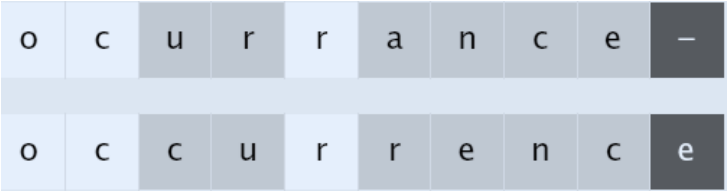
\includegraphics[width=\linewidth]{figures/edit-distance-example-1.png}
            \caption{6 replacements, 1 deletion}
        \end{subfigure}
        \hfil%
        \begin{subfigure}[ht!]{0.33\linewidth}
            \centering
            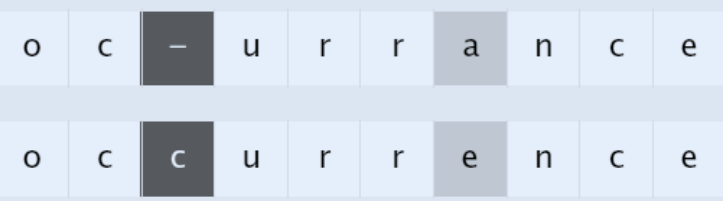
\includegraphics[width=\linewidth]{figures/edit-distance-example-2.png}
            \caption{1 replacement, 1 deletion}
        \end{subfigure}
    \end{figure}
\end{example}

\begin{listu}
    \item \textbf{input}

    \begin{listu}
        \item Strings $X = x_1 x_2 \dots x_m$ and $Y = y_1 y_2 \dots y_n$.
        \item Cost $d(a)$ of deleting symbol $a$.
        \item Cost $r(a, b)$ of replacing symbol $a$ with symbol $b$.
        
        We assume $r(a, b) = r(b, a)$ and $r(a, a) = 0$, for all $a, b$.
    \end{listu}

    \item \textbf{Goal}

    Compute the minimum total cost for matching $X$ and $Y$.
\end{listu}

\subsection{Dynamic Programming Solution}

\subsubsection{Optimal Substructure}

\begin{listu}
    \item \textbf{Goal:} match $x_1, \dots, x_m$ with $y_1, \dots, y_n$.

    \item Consider the last symbols $x_m$ and $y_n$.

    \item There are three options:
    
    \begin{listu}
        \item {\color{lightBlue}Delete} $x_m$, and optimally match $x_1, \dots, x_{m - 1}$ with $y_1, \dots, y_n$.
        \item {\color{lightBlue}Delete} $y_n$, and optimally match $x_1, \dots, x_m$ with $y_1, \dots, y_{n - 1}$.
        \item {\color{darkGreen}Match} $x_m$ and $y_n$, and optimally match $x_1, \dots, x_{m - 1}$ with $y_1, \dots, y_{n - 1}$.
        \begin{listu}
            \item We increase the cost by $r(x_m, y_n)$ if $x_m \ne y_n$.
            \item Recall that $r(a, a) = 0$, so we don't increase the cost if $x_m = y_n$.
        \end{listu}
    \end{listu}

    \item Hence in the dynamic programming, we need to compute the optimal solutions for matching prefixes of $X$ and $Y$, $x_1, \dots, x_i$ and $y_1, \dots, y_j$.
\end{listu}

Let $E[i, j]$ be the distance between $x_1, \dots, x_i$ and $y_1, \dots, y_j$. Then, \[
    E[i, j] = \begin{cases}
        0                 & \text{if } i = 0 \text{ and } j = 0 \\
        B                 & \text{if } i = 0 \text{ and } j > 0 \\
        A                 & \text{if } i > 0 \text{ and } j = 0 \\
        \min\{ A, B, C \} & \text{otherwise}
    \end{cases}
\] where \[
    \begin{aligned}
        A & = d(x_i) + E[i - 1, j]          \\
        B & = d(y_j) + E[i, j - 1]          \\
        C & = r(x_i, y_j) + E[i - 1, j - 1]
    \end{aligned}
\]

\subsubsection{Running Time}

There are $\mathcal{O}(m \cdot n)$ entries to evaluate, and each entry takes $\mathcal{O}(1)$ time to evaluate. Hence, the running time is $\mathcal{O}(m \cdot n)$.

\subsubsection{Space Optimization}

The current solution uses $\mathcal{O}(m \cdot n)$ space. However, we can optimize the space complexity of the dynamic programming solution by using a bottom up approach. 

\begin{listu}
    \item While computing $E[\cdot,j]$, we only need to store $E[\cdot,j]$ and $E[\cdot,j-1]$, so the additional space required is $\mathcal{O}(m)$.
    \item By storing two rows at a time instead, we can make it $\mathcal{O}(n)$.
    \item Usually, we include the storage of inputs, so both are $\mathcal{O}(m + n)$.
\end{listu}

However, this is not enough if we want to compute the actual solution. \href{https://en.wikipedia.org/wiki/Hirschberg%27s_algorithm}{Hirschberg's algorithm} is a space-optimized version of the dynamic programming solution that can compute the actual solution in $\mathcal{O}(m + n)$ space.

% TODO: Hirschberg's algorithm

\section{The Traveling Salesman Problem}

\subsection{Problem Definition}

\begin{listu}
    \item A complete graph $G = (V, E)$ with distance $d_{i, j}$ from vertex $i$ to vertex $j$.
    
    Note that the input needs to satisfy the triangle inequality: $d_{i, j} \le d_{i, k} + d_{k, j}$ for all $i, j, k$.

    \item \textbf{Goal:} find the shortest cycle that visits every vertex exactly once. This is called the \term{Hamiltonian cycle}.
\end{listu}

We start at node $v_1 = 1$, and want to visit other nodes in some order, say $v_2, v_3, \dots, v_n, v_1$. The total distance is \[
    d_{1, v_2} + d_{v_2, v_3} + \dots + d_{v_{n-1}, v_n} + d_{v_n, 1},
\] and we want to minimize this.

The na\"ive approach is to consider all possible Hamiltonian cycles and choose the shortest one. However, this approach has a running time of $(n - 1)! = \theta\left( \sqrt{n} \left( \frac{n}{e} \right)^n \right)$ by Stirling's approximation, which is not feasible for large $n$.

\subsection{Dynamic Programming Solution}

Consider $v_n$, the last node before returning to $v_1 = 1$. If $v_n$ is some node $c$, we find the optimal order of visiting nodes $2, 3, \dots, n$ that ends at $c$. To do so, we need to keep track of the subset of nodes visited so far, and the last node visited.

{~~~}

Let $OPT[S, c]$ bethe minimum total travel distance when starting at $1$, visiting each node in $S$ exactly once, and ending at $c \in S$. We can find the best ending node $c$ by computing \[
    \min_{c \in S} \{ OPT[S, c] + d_{c,1} \} \qquad \text{where } S = \{2, 3, \dots, n\}.
\] The Bellman equation is \[
    OPT[S, c] = \begin{cases}
        d_{1, c}                                                                & \text{if } S = \{ c \} \\
        \displaystyle
        \min_{m \in S \setminus \{c\}} ( OPT[S \setminus \{c\}, m] + d_{m, c} ) & \text{if } |S| > 1     \\
    \end{cases}
\] which yields the optimal solution \[
    \text{Final solution} = \min_{c \in \{ 2, \dots, n \}} \{ OPT[{2, \dots, n}, c] + d_{c, 1} \}.
\]

\subsubsection{Running Time}

There are $\mathcal{O}(n \cdot 2^n)$ entries to evaluate, and each entry takes $\mathcal{O}(n)$ time to evaluate. Hence, the running time is $\mathcal{O}(2^n \cdot n^2)$.

\subsection{Space Optimization}

The space complexity of the dynamic programming solution is $\mathcal{O}(n \cdot 2^n)$, which is the same as implementing the solution na\"ively. However, we can optimize by using a bottom up approach, as we do not need the entire table at any given time -- computing the optimal solution with $|S| = k$ only requires storing the optimal solution with $|S| = k - 1$. By doing so, we can reduce the space complexity to approximately \[
    \mathcal{O} \left( n \cdot \binom{n}{n/2} \right) \approx \mathcal{O} \left(  \right).
\]

\section{Remarks}

High-level steps in designing a DP algorithm
\begin{listu}
    \item Focus on a single decision in optimal solution. Typically, this is the first or the last decision. 

    \item For each possible way of making that decision, [optimal substructure] write the optimal solution of the problem in terms of the optimal solutions to subproblems

    \item Generalize the problem by looking at the type of subproblems needed. 
    
    For example, in the edit distance problem, we realize that we need to solve the problem for prefixes $(x_1, \dots, x_i)$ and $(y_1, \dots , y_j)$ for all $(i,j)$

    \item Write the Bellman equation, cover your base cases 

    \item Think about optimizing the running time/space using tricks. This is often easier in the bottom-up implementation
\end{listu}
